\documentclass[11pt,preprint,flushrt]{aastex}
%\usepackage{natbib}
\usepackage{amsmath}
\usepackage{amssymb}
\usepackage{latexsym}
\usepackage{cancel}
\usepackage{verbatim}
\usepackage{indentfirst}
\usepackage{multirow}
\usepackage{color}
\usepackage{graphicx}
\usepackage{multicol}
\usepackage{hyperref}
\usepackage{graphicx}

\usepackage{lineno}
\linenumbers

%\usepackage[utf8]{inputenc}
 
%\setlength{\arrayrulewidth}{1mm}
%\setlength{\tabcolsep}{18pt}
%\renewcommand{\arraystretch}{1.5}


\begin{document}


\newcommand {\gs} {{\tt{GalSim}}}  
\newcommand {\wf} {WFIRST}  
\newcommand {\wfa} {WFIRST}  
\newcommand {\optical} {{\tt{OpticalPSF}}} 
\newcommand {\gauss} {{\tt{Gaussian}}} 

%\def\dv{\mbox{$\Delta V$}}

%\title{Voltage non-linearity effects on \wfa\ PSF profiles for weak lensing measurements using {\tt{GalSim}} simulations}
\title{The effect of detector nonlinearity on \wfa\ PSF profiles for weak gravitational lensing measurements}
\author{A. A. Plazas$^{\dagger a}$, C. Shapiro$^{a,b}$, A. Kannawadi$^c$, R. Mandelbaum$^c$, J. Rhodes$^{a,b,d}$, $\&$ R. Smith$^b$  }
\email{$^\dagger$Andres.A.Plazas.Malagon@jpl.nasa.gov}
\affil{$^a$Jet Propulsion Laboratory, California Institute of Technology, 4800 Oak Grove Dr., Pasadena, CA 91109, USA}
\affil{$^b$California Institute of Technology, 1200 E. California Blvd., CA 91125, USA}
\affil{$^c$McWilliams Center for Cosmology, Department of Physics, Carnegie Mellon University, Pittsburgh, PA 15213, USA}
\affil{$^d$Institute for the Physics and Mathematics of the Universe, 5-1-5 Kashiwanoha, Kashiwa, Chiba Prefecture 277-8583, Japan }
\begin{abstract}

Weak gravitational lensing (WL) is one of the most powerful techniques to learn about the dark sector of the universe. To extract the WL signal from astronomical observations, galaxy shapes must be measured and corrected for the point spread function (PSF) of the imaging system with extreme accuracy. Future WL missions (such as NASA's Wide-Field Infrared Survey Telescope, WFIRST) will use a family of hybrid near-infrared CMOS detectors (HAWAII-4RG) that are untested for accurate WL measurements.  Like all image sensors, these devices are subject to conversion gain nonlinearities (voltage response to collected photo-charge) that tend to attenuate bright objects such as reference stars that are used in PSF determination.
We study this type of detector nonlinearity (NL) and show how to derive requirements on it from \wf\ PSF size and ellipticity requirements. We simulate the PSF optical profiles expected for \wf\, 
and measure the fractional error in the PSF size ($\Delta R/R$) and the absolute error in the PSF ellipticity ($\Delta e$) as a function of parameters such as the expected magnitude of typical stars in \wf\ and the NL model parameters. 
We find that, uncalibrated, NL can induce an error of $\Delta R/R=2.5\times 10^{-3}$ and $\Delta e_2=5\times 10^{-4}$ in the PSF size and ellipticity in the H158 bandpass for the expected brightest stars in \wf.  In addition, our simulations show that to limit the bias of $\Delta R/R$ and $\Delta e$ in the H158 band to $\sim 10\%$ of the estimated \wf\ error budget, the mean NL parameter $\beta$ must be calibrated to $\sim3.5\%$ and $\sim 10\%$, respectively. 
\end{abstract}

\section{Introduction}
Weak gravitational lensing (WL) has been identified as a powerful probe of the nature and evolution of the components of the Universe. In particular, \emph{cosmic shear}\textemdash the subtle  distortions of background galaxy shapes by the large-scale structure of the Universe\textemdash constrains the properties of dark matter and dark energy through the measurement of the expansion history and growth of structure of the Universe \citep{refregier03, hoekstra08, kilbinger15}. WL measurements also allow to test the validity of General Relativity that relates the gravitational potential to the matter-energy distribution. Several surveys in the visible part of the spectrum  of $>1000$~deg$^2$ of the sky are currently underway and use the WL signal from hundreds of millions of galaxies as one of their central scientific techniques (\emph{e.g.}, the Dark Energy Survey (DES), \citealt{diehl12}, \citealt{jarvis15}; the Kilo-Degree Survey (KiDS), \citealt{kuijken15}; and the Hyper Suprime-Cam Survey (HSC), \citealt{miyazaki12}). In addition, future ground- and space-based surveys and missions in the visible and near infra-red (NIR) are planned to image more than O($10^9$) galaxies in the next decade (\emph{e.g.}, the Large Synoptic Survey Telescope (LSST), \citealt{ivezic08}; the Euclid spacecraft, \citealt{laureijs11}; and NASA's Wide-Field Infrared Survey Telescope (WFIRST), \citealt{green12}, \citealt{spergel13}, \citealt{spergel15}).

The process of extracting the WL signal from images of the sky, in the presence of intrinsic galaxy ellipticity variations that are $\sim$ 0.4 r.m.s, is highly non-trivial. It must be done through a statistical analysis of large galaxy samples, with a careful control of systematic uncertainties. The dominant signal produced by WL can be described by a local linear transformation of the source image that produces a shear (a complex, spin-2 field of components $\gamma_1$ and $\gamma_2$) and a scalar magnification, both of which have an r.m.s. amplitude of only $\sim 2 \%$ in the case of cosmic shear. Most of the background galaxies usable by WL are at hight redshift (with low signal-to-noise (S/N) ratio) and with a size comparable or smaller than the Point Spread Function (PSF) of the imaging system. Incorrect estimation of the size of the PSF induce a modulation in the signal (multiplicative errors), and errors in the estimation of the PSF ellipticity propagate into asymmetries that produce coherent spurious patterns (additive errors) that mimic the WL signal. Bright stars are commonly used to estimate the PSF, and then this information must be interpolated to the observed galaxy positions to deconvolve the PSF contribution and measure the galaxy shape (in the form of a complex ellipticity $e=e_1 + i e_2$) to estimate the shear field.\footnote{Most of the shape measurement algorithms to date rely on the accurate measurements of galaxy shapes to produce an estimator of the WL shear field $(\gamma_1, \gamma_2)$. However, recent algorithms propose skipping this step and creating a direct shear estimator through Bayesian analysis (\citealt{bernstein14}, \citealt{bernstein15}, \citealt{schneider15}).} This interpolation step is subject to introduce systematic errors if the information inferred from the stars does not fully constrain the PSF at the galaxy position with the required accuracy. In order not to bias the determination of cosmological parameters and dark energy for Stage IV surveys (in the language of \citealt{albrecht06}), the ellipticity and size of the PSF must be known to an accuracy of O(10$^{-3}$) (\citealt{huterer06}, \citealt{amara08}, \citealt{paulin08}, \citealt{paulin09}, \citealt{massey13}, \citealt{cropper13}) or better ($4.7 \times 10^{-4}$ for the knowledge of the \wfa\ PSF ellipticity, \citealt{spergel13}).

%Space-based measurements offer potentially enormous advantages for weak lensing because of high angular resolution and stability of the observing platform, allowing accurate characterization of the instrumental point spread function (PSF).

Systematic errors that originate from a telescope's detectors (image sensors) can introduce biases in astronomical observables such as photometry and astrometry that propagate into shear measurement biases. These type of errors have been extensively studied in the case of thick, fully-depleted, high-resistivity Charge Coupled-Devices (CCDs), which are the detectors of choice for many current and planned surveys such as DES, HSC, and LSST (\citealt{stubbs14}, \citealt{plazas14}, \citealt{gruen15}). It is of great importance to quantify the impact of these sensor effects on the inference of cosmological parameters, in particular through WL (\citealt{jarvis14}, \citealt{mandelbaum14b}, \citealt{meyers14}). Future missions such as the James Webb Space Telescope and \wfa\ will utilize a new family of near-infrared detectors that are also subject to effects such as nonlinearity, reciprocity failure (\citealt{bohlin05}, \citealt{biesiadzinski11}), interpixel capacitance (IPC) (\citealt{mccullough08}, \citealt{kannawadi15}), and persistence (\citealt{smith08}). These effects can potentially imprint biases on weak lensing shape measurements if not taken into account. 

In this paper we study the effect of nonlinear detector conversion gain (voltage response to collected photo-charge) on PSF size and ellipticity in the context of the NIR detectors that will be used by NASA's \wf\ mission. This type of detector nonlinearity (NL) will tend to attenuate the measured flux in bright stars and broadening the inferred PSF. In other words, NL preferentially depresses the flux in the core of the PSF relative to the wings, thus complicating its deconvolution from the observed galaxy image, which itself is fainter and less subject to the effects of NL. In addition, even though NL does not induce a spurious ellipticity by itself, it modifies the ellipticity if the PSF is anisotropic. Our analysis is also useful to set preliminary requirements on NL for these sensors. Once characterized, NL can be corrected in each image, and remaining residuals will depend on the accuracy in the knowledge of the NL parameters and their spatial variation. We use the {\tt{python}}/{\tt{C++}} code \gs\footnote{\url{https://github.com/GalSim-developers}, \url{https://wfirst.ipac.caltech.edu/sims/Code.html}} \citep{rowe15} to create PSF profiles with the optical properties of \wfa\ to analyze the impact of NL on PSF size and ellipticity. 

In Section \S2 we summarize the main characteristics of the NIR detectors that will be used in \wfa\, and describe NL. In Section \S3 we describe the simulations we create to study NL for \wfa\ PSF profiles. Section \S4 presents our main results on fractional errors in size and absolute errors in ellipticity caused by NL, as function of relevant parameters such as the model parameters and PSF magnitude. We also study the effect of the spatial variability of the NL model parameter $\beta$ along the pixel array. We conclude in Section \S5 with a discussion of our results and how they can be used in the derivation of NIR detector specifications to satisfy WL accuracy requirements.  

\section{Voltage nonlinearity in the NIR detectors of \wfa}
\label{section:NL}
%\textcolor{black}{In this section we explain voltage non-linearity, and how it can affect WL science through PSF broadening. Cite the appropriate references from the literature (i.e., previous studies of NL for these type of detectors). Roger's document on measurements and emails have many good explanations, and should be cited/paraphrased.}

%% There is an obvious potential for non-linearity between photon ?ux and output voltage in the photovoltaic detectors which is absent in CCDs, simply because the detector capacitance is not �xed, but does in fact depend on the width of the pn depletion region, which in turn depends on the value of the reverse bias voltage. (Variations in the size of the depletion region do occur in a CCD, but this is a small e??ect.) The bias voltage changes continuously as the cell integrates, irrespective of whether it is storing photogenerated charges or dark current charges.

%In general, how- ever, IR arrays are continuously exposed to light, and therefore the exposure time is controlled by the sequence of reset and read pulses.

% Sample Up The Ramp: 
%In this approach, the signal is sampled many times at regular intervals throughout the duration of the exposure, rather than multiple times at the beginning and at the end. Therefore, the signal can be seen to ``ramp'' up (Chapman et al., 1990; Garnett and Forrest, 1993)

%Each pixel of an HxRG array is a 3-T (three transistor) design with a source fol- lower MOSFET providing charge-to-voltage conversion.  The gate of the source fol- lower is connected to the detector pixel with an indium bump

%IPCInter-pixel capacitance (IPC): For CMOS arrays made with source follower (SF) pixels, the gate of the SF of one pixel is capacitively coupled to some degree to the SF in each of the 4 neighboring pixels. Since the voltage on a SF gate changes as photocharge is accumulated, this voltage change will modify the voltage on neighboring pixels, causing an electrical crosstalk between pixels. This crosstalk occurs after charge collection and during the charge-to-voltage conversion pro- cess. This ?inter-pixel capacitance? (IPC) can be conducted via three paths: (1) through the ROIC, (2) through the indium bumps, or (3) through the detector ma- terial. Since a silicon PIN detector is fully depleted, capacitive coupling through the detector material is dominant. For a H2RG, the IPC for a silicon HyViSI H2RG array is 8-10% to nearest neighbor.

%Non-linearity: A source follower is inherently non-linear, since the gate of the amplifier de-biases during charge integration. This leads to a roll-off of response as the detector approaches full well. Pixel full well is typically defined as the charge level at which the response is 5% deviation from linear, which is typically about 100,000 electrons for the HxRG designs (the exact number depends on the operating conditions)

The \wfa\ mission will use a 2.4 m telescope equipped with a Wide Field Instrument (WFI) with 6 bandpass filters: Z087, Y106, J129, W149, H158, and F184 (\citealt{spergel15}).\footnote{In addition to a integral field unit and a coronagraph for supernovae and exoplanet studies, respectively.} The WFI will perform a high-latitude survey (HLS) over an area of 2200 deg$^2$ in four NIR ($\sim0.92$\textendash $2.00\ \mu$m) bands (Y106, J129, H158, and F184) down to a 5$\sigma$ point-source AB magnitude of 26.7 in the J129 band. The weak lensing program in the HLS will measure shapes of about 380 million galaxies in the J129, H158, and F184 bands (\citealt{spergel15}). 

The WFI possesses a wide-field channel that has a Focal Plane Assembly (FPA) of 18 4k$\times$4k HgCdTe (mercury, cadmium, and telluride) NIR detectors, arranged in a 6x3 layout and with a pixel size and scale of 10 $\mu$m and 0.11 arcseconds per pixel, respectively. The HgCdTe NIR detectors are manufactured by Teledyne Imaging Systems, and are part of a family of detectors known as HXRG\footnote{``HAWAII X$k\times$ X$k$ pixels with Reference pixels and Guide mode", where ``HAWAII" stands for HgCdTe Astronomical Wide Area Infrared Imager.}. 

The detector arrays are fabricated with a hybrid complementary metal-oxide-semiconductor (CMOS) architecture, which combines the qualities of HgCdTe to detect infra-red light (\emph{e.g.}, altering the relative molar contributions of mercury and cadmium allows to tune the band gap up to an order of magnitude) and the advanced readout performance of integrated circuits. Light is absorbed, converted to charge through the photoelectric effect, and collected by electric fields generated by a reverse-biased p-n junction in the detector layer.  The charge per pixel is then converted to a voltage and amplified through a source follower. This operation is performed in the silicon readout integrated circuit (ROIC) layer, which is connected to the HgCdTe detection layer by indium interconnects (one bump per pixel). Finally, the ROIC transfers the signal (and for this it is also known as ``multiplexer") to the off-chip electronics at the edge of the FPA, where it is digitized through analog-to-digital converters \citep{beletic08}.

%The presence of the signal amplifier in each pixel causes a signal coupling among neighboring pixels (\emph{i.e.}, the charge in a pixel induces a voltage change in a neighbor) that is known as Inter-Pixel Capacitance (IPC). IPC is a type of crosstalk analogous to the amplifier crosstalk seen in multichannel CCDs (REFERENCE to O'Connor et al), and can have undesirable effects on PSF correction for WL science (REF ARUN et al). In addition to IPC, NIR detectors present other type of sensor effects that must be calibrated and/or corrected for accurate WL measurements. In particular,  

An ideal detector would produce a measurable signal that is proportional to the detected photons. However, there are several places in the signal chain where this expected linearity is not realized, and the conversion of charge to measured voltage (or digital numbers) becomes non-linear. First of all, the charge accumulation rate might be a function of the photon-accumulation rate. This type of effect is known as reciprocity failure (RF), and it is a flux-dependent type of nonlinearity (\citealt{smith08}, \citealt{biesiadzinski11}). In addition to RF, each pixel's p-n junction acts as a parallel-plate capacitor, and as charge accumulates the depletion region narrows, causing a deviation from linearity of the charge-to-voltage conversion relation. Nonlinearity can also be introduced through the electronic gain of the ROIC. 
The last two types of nonlinearity depend on fluence (total flux per pixel, or integrated signal, as opposed to RF, which is flux dependent), and can be analyzed together in a singe transfer function typically called ``nonlinearity" (NL). We study the impacts of NL (more relevant at high signals) on PSF measurements in this paper, while we leave investigations on the consequences of RF (relevant at lower signals) on WL measurements for future work. 

Assuming that the dominant contribution to nonlinearity is the varying capacitance of the pixel p-n junction, the correction to the detector signal is well approximated by a quadratic term:
\begin{align}
S(Q)= Q + \beta Q ^2 % (\mathrm{e^-})
%\textcolor{blue}{Following \citealt{hilbert04}, \citealt{hilbert08}, and \cite{hilbert14} (which study non-linearity in the Hubble Space Telescope's Wide Field Camera (WFC3) NIR detector\textemdash a H1RG 1.7 $\mu$m cutoff detector, similar to the H4Rg that will be used in WFIRST), we model the measured voltage $S$ corresponding to the number of electron-hole pairs $Q$ as a fourth-order polynomial of the form:}
%To obtain a functional model of NL as a function of signal, we use laboratory measurements\footnote{Performed at Caltech by R. Smith and collaborators.} of H2RG 1.7 $\mu$m cutoff detectors, which have the same basic design of the H4RG that will be used in the WFI but with 18 $\mu$m pixels. A constant flux source is illuminated on the detector, and the NL measurements are done by non-destructive sample-up-the-ramp (SUTR) readout at multiple times. The value of the first frame is subtracted, and then the \emph{mean} signal is fitted to a polynomial. These measurements show that the voltage relation for a measured signal $S$ is well fit by a quadratic function in the signal $Q$ of the form:
%\begin{align}
%S(Q)= Q + \beta Q ^2  (\mathrm{e^-}) 
\label{NL}
\end{align}
Here, $Q$ is the true number of elementary charges collected in the pixel, $S$ is the number inferred from the voltage change at the sense node, and $\beta$ is a constant.  To estimate $\beta$, we compute $Q(V)=C(V)*V/q_e$, where the total capacitance is given by the varying junction capacitance plus a constant $C(V) = C_{\rm jn}(V) + C_{\rm fix}$. \textbf{[CITE McCAUGHREAN]}  The junction capacitance varies as
\begin{equation}
C_{\rm jn}(V) \sim (1+V/V_{bi})^{-1/2}
\end{equation}
Here, $V_{bi}$ is the ``built in'' potential of the junction and $V=V_{\rm DSUB}-V_{\rm RESET}+\delta V$, where $V_{\rm DSUB}$ is the constant potential at the diode cathode, $V_{\rm RESET}$ is the initial potential at the anode, and $\delta V$ is the change in anode potential due to accumulated photocharge.  As an example, we plug in measurements of a 2.4$\mu$m cutoff H2RG by Finger (2006): \textbf{[CITE FINGER]}% https://www.eso.org/sci/meetings/2006/neon-2006/Finger.pdf
\begin{eqnarray*}
V_{\rm bi} &=& 0.412{\mbox V} \\
V_{\rm DSUB} &=& 1{\mbox V} \\
V_{\rm RESET} &=& 0.5{\mbox V} \\
C_{\rm fix} &=& 17.8 {\mbox fF} \\
C_{\rm jn}(V=.912{\mbox V}) &=& 30 {\mbox fF}
\end{eqnarray*}�
Using these parameters to compute $Q(V)$ for $ 0\le \delta V \le 0.3$ V (corresponding to maximum $Q$=60115) and then inverting to find $S(Q)$, we find it is well-fit (to 0.1\% or better) by (\ref{NL}) with $\beta$=-1.18e-6.  In practice, HxRG calibrations have included additional polynomial parameters to reduce residuals, extend the range of valid $Q$, and account for additional nonlinear effects \textbf[CITE HILBERT PAPERS]; however, the additional parameters are highly degenerate, resulting in large variances in the fitted values.  For our purposes, it suffices to analyze the shape-distorting effects of nonlinearity using a single parameter, $\beta$, which encapsulates most of the effect.

%\textcolor{blue}{Following \citealt{hilbert04}, \citealt{hilbert08}, and \cite{hilbert14} (which study non-linearity in the Hubble Space Telescope's Wide Field Camera (WFC3) NIR detector\textemdash a H1RG 1.7 $\mu$m cutoff detector, similar to the H4Rg that will be used in WFIRST), we model the measured voltage $S$ corresponding to the number of electron-hole pairs $Q$ as a fourth-order polynomial of the form:}
%To obtain a functional model of NL as a function of signal, we use laboratory measurements\footnote{Performed at Caltech by R. Smith and collaborators.} of H2RG 1.7 $\mu$m cutoff detectors, which have the same basic design of the H4RG that will be used in the WFI but with 18 $\mu$m pixels. A constant flux source is illuminated on the detector, and the NL measurements are done by non-destructive sample-up-the-ramp (SUTR) readout at multiple times. The value of the first frame is subtracted, and then the \emph{mean} signal is fitted to a polynomial. These measurements show that the voltage relation for a measured signal $S$ is well fit by a quadratic function in the mean signal $\langle Q \rangle$ of the form:
%\begin{align}
%\hat{p} = \frac{\frac{\partial I}{\partial p} C^{-1} (I - I_{p=0})} {\frac{\partial I}{\partial p} C^{-1} \frac{\partial I}{\partial p}} \\
%\end{align}
%To determine the scale of spatial variation in NL among the individual pixels, high S/N co-added flats were taken at different exposure times and constant flux, and their ratios taken (after subtraction of a mean dark flat for each frame). The sequence of means of the ratio images followed the quadratic function of Eq. \ref{NL}, with a standard variation that includes shot noise and deviations of the individual NL curves from the mean NL. After subtracting in quadrature the contribution from shot noise, a remaining floor in the variation of about $12\%$ r.m.s. can be attributed to the variation of the NL coefficient $\beta$.  
%\textcolor{blue}{For the pixels in the WFC3 NIR detector, \citealt{hilbert14} calculate that $\beta \in [-0.5,1.5]\times10^{-6}$, $\gamma \in [-1,0.5]\times10^{-10}$, and $\delta \in [-1,2]\times10^{-15}$. Therefore, in our calculations we use the midpoints these intervals as nominal values for each parameter, \emph{i.e.} $(\beta_0$, $\gamma_0$, $\delta_0$) = ($0.5\times10^{-6}$, $-0.25\times10^{-10}$, $1.5\times10^{-15}$). In addition, we will assume that the coefficients in each pixel can be drawn from a Gaussian distribution with means $(\beta_0$, $\gamma_0$, $\delta_0$) and ($\sigma_{\beta}$, $\sigma_{\gamma}$, $\sigma_{\delta}$) = ($5.9\times10^{-7}$, $5.625\times10^{-11}$, $1.35\times10^{-15}$)  (dispersion values taken as the mean of the standard deviations calculated in four cuadrants of the WFC3 H1RG detector by \citealt{hilbert08})}

%Thus, in our calculations we assume that each individual pixel satisfies a NL function of the same form as Eq. \ref{NL}. In addition, when we study the impact of spatial variation of the model coefficient along the pixel array we will assume that the parameter $\beta$ in each pixel can be drawn from a Normal distribution of the form $\mathcal{N} \sim (\beta_0,\ \sigma_{\beta_0})$, where the nominal mean value $\beta_0$ is measured to be $-3.566\times10^{-7}$/e$^{-}$. 

%This mean nominal value implies an attenuation of the signal of about $4\%$ for 
For this work, we assume a typical pixel full well depth in the WFI detectors of $1.1 \times 10^5$ electrons (Eq. \ref{NL}).  
Using PSF profiles with a simulated AB magnitude up to 18.3 for an exposure time of 168.1 seconds (expected for the HLS), the total flux in each band is shown in Table 1, along with the peak pixel value. When the profile is drawn on a pixelated postage stamp with a scale of $p=0.11$ arcseconds and placed on the center of the pixel\footnote{Note that the peak value is a function of the PSF profile centroid location within the pixel, as well as resolution. When drawing the PSF profiles in our simulations, we randomize the PSF centroid within the native scale pixel, as described in Section YYY.}, this particular magnitude produces a peak charge of $\sim 1e5$e$^{-}$ (Y106 band, see Table 1), which represents about 90\% of the typical pixel full well value assumed above.
\textbf{[CALCULATE NL \% for nominal beta]}
%which represents a total flux (over all pixels of the postage stamp where each profile was drawn) of up to $\sim 2.82 \times 10^5 \ \mathrm{e^-}$ (J129 band, see Table 1), with a resulting in a signal attenuation of about $3.4\%$.  
Calculations with the {\tt{Trilegal}} galaxy model\footnote{\url{http://stev.oapd.inaf.it/cgi-bin/trilegal}} \citep{girardi12} show that there will be approximately 20 stars at or brighter than this magnitude and flux level per detector.\footnote{We thank Christopher Hirata, who performed these calculations. The NIR filter sets used in {\tt{Trilegal}} had to be converted from the vega to the AB magnitude system. The code was run at the South Galactic Pole with the SDSS and 2MASS ($ugriz$ and $JHK_\mathrm{s}$) filters in 1 deg$^2$ and interpolated to WFIRST filter centers, which ignores the fact that stars have spectral structure in the NIR, but gives a result good to about $10\%$. The number of stars quoted in the text is expected to be higher at moderate galactic latitudes.} 
% (Be aware that many of the NIR filter sets in Trilegal are on the Vega system and have to be converted to AB.) I did a run at the South Galactic Pole with the SDSS + 2MASS (ugriz + JHKs) filters in 1 deg^2 and interpolated to WFIRST filter centers. [This isn't really a great procedure since the stars have spectral structure in the NIR, but at the "tens of percents" level -- which I think is what you're asking for -- this should be fine.] In 1 deg^2, I get 964 saturated stars in J, 943 in H, and 667 in F184. This corresponds to 15.0, 14.7, and 10.4 saturated stars per detector. At moderate Galactic latitude, these numbers will be higher. Also each detector will have a software-defined guide window that will be placed on one of the stars that would saturate in the full-length exposure.}  }  
We assume that galaxies will have about two orders of magnitude fewer total electrons than bright stars, and therefore for this quadratic model, star shapes are distorted by NL and galaxies are (approximately) not, which would result in an incorrect PSF correction if not accurately calibrated. We apply this mapping to simulated \wfa\ PSF profiles and quantify the impact on PSF properties such as size and shape. 
%We have verified that the results using the mean NL coefficient for all pixels do not differ significatively from those using the distribution above for each pixel (see Section and Table 2 below). 
% DC offsets which are intrinsic to the readout circuit and which vary from pixel to pixel

\section{Methods}
\label{methods}
\subsection {Simulations}
We use the publicly available {\tt{GalSim}} code (v1.3) to simulate the impact of NL on the \wfa\ PSF shape and size. {\tt{GalSim}} is a {\tt{python/C++}} open-source code that allows the user to create simulations of astronomical objects, and it is especially useful in weak lensing investigations. 

\citet{kannawadi15} have developed within \gs\ v1.3 a \wfa\ module called ``{\tt{galsim.wfirst}}", which allows the simulation of a PSF profile according to the optical design characteristics of the \wfa\ WFI \citep{pasquale14}\footnote{\citealt{pasquale14} discuss the so-called ``Cycle 4" optical design, whereas the \gs\ \wfa\ module -used in this work- uses files corresponding to ``Cycle 5".} through the calling of the {\tt{galsim.wfirst.getPSF}} routine. 
This routine returns a {\tt{python}} dictionary %of {\tt{galsim.ChromaticOpticalPSF}} objects
indexed by each one of the 18 H4RG detectors of the FPA. It uses the optical configuration of the pupil plane\footnote{The pupil plane configuration is not circular in all the bands but the simulated PSFs use circular apertures.} to simulate PSF images in any \wfa\ WFI bandpass filter, with expected optical aberrations approximated as a linear combination of Zernike polynomials (up to Noll order equal to $11$, \citealt{noll67}). For this work, we have created simulations in the four bands of the HLS.  A central circular obscuration ($30 \%$) and six support struts are included as well. The pupil plane configurations and Zernike models are publicly available.\footnote{\url{http://wfirst.gsfc.nasa.gov/science/sdt_public/wps/references/instrument/}} 

The current version of the module does not include PSF variations across the detector field of view, and the PSF returned corresponds to that at its center. In addition, the module assumes that the pupil plane configuration of all the six bands is the same and equivalent to that of the ``red" bands (\emph{i.e.}, W149, H158, and F184), and that the struts are not, in general, radial nor evenly spaced. %However, these last two assumptions can be relaxed to expedite calculations, and the optional keyword {\tt{approximate\char`_struts}} can be set to {\tt{True}}. 
The module generates PSF models that do not include pointing jitter nor charge diffusion. These effects could be added to the profile (\emph{e.g.,} by means of an extra convolution with a Gaussian profile in the case of diffusion), but we did not include them in our simulations. Their effect would be to create a slightly larger PSF, reducing the impact NL. Their omission makes our results slightly conservative.  

The ellipticity of the WFI PSF varies over the field of view due to optical aberrations. To make our results conservative, we simulate only detector \#18, whose PSF was determined to have the largest ellipticity (see Section \S3.2 for a description of the shape measurement method used) across all bands among all the detectors (Table 1). We also evaluate the PSF at the mean wavelength weighted by each bandpass or effective wavelength, resulting in an (achromatic) {\tt{galsim.OpticalPSF}} object.
% and set the {\tt{approximate\char`_struts}} keyword to {\tt{False}} when creating the profile. 
We then form an effective PSF by convolving the profile with a 2D top-hat profile of length equal to the nominal angular scale of the \wfa\ WFI ({\tt{galsim.wfirst.pixel\char`_ scale$=0.11$}} arcseconds per pixel). 

%Table 1
\begin{table}[!htb]
\centering
\begin{tabular}{ |c| c | c| c| c| c| c | c| c|}
\hline
\multirow{2}{*}{Band} & Min. $\lambda$ & Max. $\lambda$ & $\lambda_{\text{eff}}$ & $b(\lambda)$ & peak value  & e$_1$ & e$_2$ & $\sigma$ (pix) \\
& ($\mu$m) & ($\mu$m) & ($\mu$m) & ($\times10^5$) (e$^{-}$) & ($\times 10^{5}$) (e$^{-}$) & (\#18) & (\#18) & (\#18)  \\
\hline 
Y106 & 0.900 & 1.230 & 1.061 & 2.7621 &  1.00237  &-0.0163  & 0.2035 & 1.7020 \\
J129  & 1.095 & 1.500 & 1.292 & 2.8267 &  0.89742 & -0.0127  & 0.1325 & 1.717 \\
H158 & 1.340 & 1.830 & 1.577 & 2.7922 &  0.38654 & -0.0089 & 0.0802 & 1.832 \\
F184 & 1.630 & 2.060 & 1.837 & 1.8346 &  0.71890 & -0.0071 & 0.0550 & 1.995 \\
\hline
\end{tabular}
\caption{The first column lists the four bands that will be used in the HLS. For weak lensing analysis, multi-band shape measurement will be done in bands J129, H158, and F184. Columns 2, 3, and 4 show their minimum, maximum, and effective wavelengths, respectively (from \citealt{kannawadi15}). Column 5 shows the baseline total flux (in electrons) $b(\lambda)$ of Eq. \ref{flux} at AB magnitude 18.3 (at 161.1 seconds of exposure time) in each band as calculated in \gs\, while column 6 shows the peak value for each profile at that same magnitude. The last three columns show the ellipticity components and size of the \wfa\ PSF profile in detector number 18 as calculated by the adaptive moments routine in \gs. Chip \#18 was found to possess the largest values of absolute PSF ellipticity.}
\label{table:1}
\end{table}

The resulting PSF profile created in this way will be undersampled (in accordance with the \wfa\ WFI design). In order to maximize the field of view, detectors in instruments of space missions are usually built with a physical size that results in undersampled images, which fail to satisfy the Nyquist-Shannon criterium for the maximum band limit set by the optical response of the system, and therefore produce aliased images.\footnote{The Nyquist-Shannon criterium states that the sampling interval $p$ must satisfy $p < 1/(2 u_{max})$, where $u_{max}$ is the highest frequency in the signal, in order to avoid aliasing.} In general, it is not possible to recover all the information of a continuous function from a discrete sample of points if the image is aliased, and measurements of astronomical object's properties such as magnitude and shape will be erroneous (\citealt{lauer99a}, \citealt{fruchter11}, \citealt{rhodes07}). Also, in particular, we found that our shape measurement algorithm fails when most light is concentrated in a few pixels.


%nonlinearity depends on the absolute pixel values, and therefore it will depend on where the star is centered within the pixels

%I think that a better representative of what we?ll see in WFIRST would be to use something like 3x3 subsampling, closer to the Nyquist limit.  In that case, you?re not so close to infinite resolution that you can ignore the impact of centroid shifts within the native pixels.  You might find that some star centroid locations are worse than others, and you can see how wide is the range - are they all close to the average, or is there a tail?

%OK, let's take a look.

%Andr�s, using the data you are currently generating, can you please make the relevant histogram?  That is:
%-choose centroid offset
%-render N=3 subsampled image
%-measure size (and ellipticity) difference between linear and nonlinear version
%-repeat for many offsets (uniformly spaced or uniform random over a native pixel) and plot e.g. the histogram of size differences

 %I repeated the histograms of the delta metrics, explicitly casting the results from hsm to double precision (by means of 'float'; although I would think hsm already returns this kind of precision). I ran 100 realizations of centroid offsets (using the same seeds for NL vs no NL), with pixel scale=0.11 and n_sub=3. All this for a WFIRST PSF at lambda 1292 nm with flux 9.5477e4. I used the nominal beta0 value.
 
To overcome this problem in real data, multiple dithered exposures are taken, and then put together by means of an image combination algorithm (\citealt{lauer99b}, \citealt{fruchter02}, \citealt{bertin06}, \citealt{rowe11}) in order to produce an oversampled image that satisfies the Nyquist-Shannon criterium. To study NL with simulations, however, we do not need to make use of such external software\textemdash which can be computationally expensive\textemdash to produce an image at higher resolution, given that the parameters of the simulated images can be fully controlled.  Instead, we render the convolved PSF profile\textemdash including the pixel response at its native scale\textemdash as a \gs\ object at a high resolution through the method {\tt{galsim.GSObject.drawImage}},\footnote{The keyword {\tt{method}} should be set to {\tt{`no\char`_pixel'}} when calling {\tt{galsim.GSObject.drawImage}}, since by default it convolves its argument profile with a boxcar of length {\tt{pixel\char`_scale}}. This extra convolution must be turned off because the effective PSF profile we create already includes this pixel response.} setting the parameter {\tt{scale}} to $p/N$, where $N$ is a positive integer and $p$ is the native pixel scale. 
 %We render the convolved PSF profile \textemdash including the pixel response at its native scale \textemdash with a resolution $p/N$, and then apply the NL effect to the image.} 
 
Defining $Q\equiv1/p\times u_{\text{max}}$ as the sampling factor ($Q<2$, $Q=2$, and $Q\geq2$ represent under-, critically, and over-sampled images, respectively), we see that in order to produce an over-sampled image ($Q\geq2$), the Nyquist-Shannon criterium implies that $N$ must be given by (see \emph{e.g.}, \citealt{marks09}, \citealt{shapiro13})
\begin{align}
N=\frac{2p}{\lambda_{min} F}
\label{nimages}
\end{align}
where $p$ is the pixel size, $\lambda_{min}$ is the shortest wavelength in a given filter, and $F$ is the the f-number of the telescope. In the case of the \wfa\ telescope, $p=10\ \mu$m and $F=7.8$, resulting in $N\geq3$ ($N\geq2$) for the J129 (H158) band. Thus, we have chosen to set $N=3$ in our simulations, which will produce a number of images similar to what the WL survey in \wf\ will use per exposure (5\textendash7 across two epochs). At this resolution, it will also be possible to study the impact of centroid shifts within the native pixels (since NL depends on the absolute pixel values it will also depend on where the star is centered within a particular pixel), and therefore for our simulations we randomly vary the PSF centroid within a pixel.

%However, we have conservatively chosen a larger $N$ for our simulations to reduce discretization errors. We have verified the convergence of our results for $N\geq6$.  
%However, we oversample the images at  the error due to discretizing, and to reduce the variance due to any sub-pixel offsets that PSFs may have. We have set $N$ equal to $6$ for our simulations.

Notice that this method to approximate oversampled images can only be used in the case of sensor effects such as NL, which only depend on each pixel individually. In the case of other effects that correlate the signal in one pixel with the signal of its neighbors (such as IPC), the effect should be applied to the native scale of the detector and then a properly sampled image should be generated through adequate combination of several dithered images before performing any analysis (see for instance the ``interleaving" algorithm of \citealt{kannawadi15}, also included in \gs). 

\begin{figure}[!ht]
\centering
\resizebox{\hsize}{!}{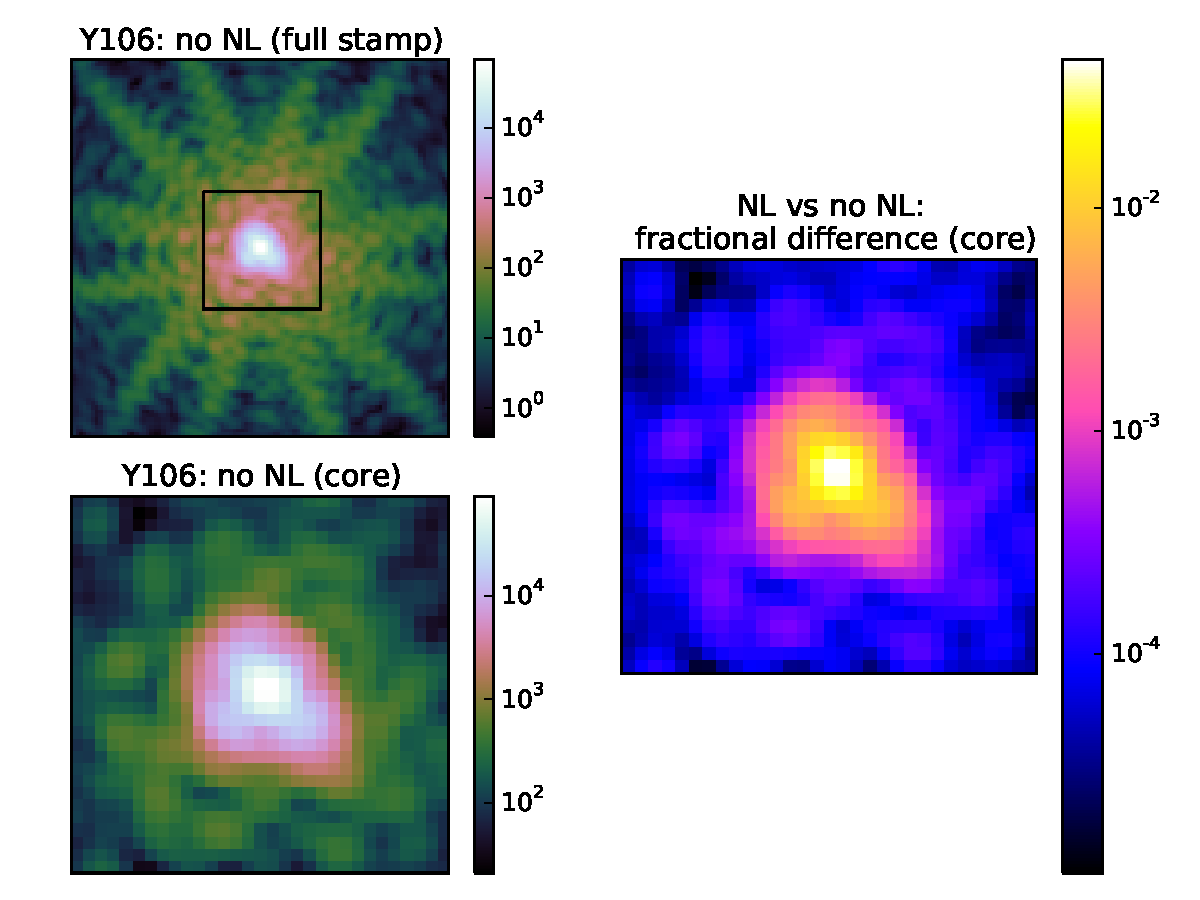
\includegraphics[page=1]{plots/f1.eps}}
\caption{Example of the \wfa\ PSF profiles in the Y106 band created by the {\tt{galsim.wfirst.getPSF}} method. The profile is drawn on a postage stamp with a size of $1.5k \times1.5k$ pixels ($k=64$) and a resolution of $p/N$, with $p=0.11$ arcseconds and $N=3$. Before drawing the profiles, they are first convolved with a pixel response of size $p$ and given a flux obtained through the use of the {\tt{galsim.wfirst.getBandpasses (AB\char`_zeropoint=True)}} routine at an AB magnitude of 18.3. However, to preserve the correct response to NL, the higher-resolution image has $N^2$ more total flux. The NL effect is applied at the native pixel scale $p$, and the centroid of the profile randomized within the pixel at this same scale (in this example the centroid and the pixel center coincide). The upper left panel shows the full postage stamp PSF image without the NL applied, while the lower left panel shows a zoom into the core (squared central region in upper left panel) of 30 by 30 high resolution pixels. The right-hand side image shows the fractional difference between the PSF without the NL applied and a PSF with NL using $\beta_0$ for the model parameter.} 
%is of the order of 1\% in the core pixels which have more flux, and it is better seen in the right-hand side image.}
\label{f1?}
\end{figure}

The PSF profiles are drawn into squared postage stamps of size $1.5k$ pixels ($k=64$), large enough to ensure that most of the flux applied to the original profile object is conserved when drawing the image. %In addition, this avoid biases in PSF determination arising from object selection and deblending. 
Each profile object was assigned a total flux of 
\begin{align}
f=b(\lambda)\times10^{0.4 (18.3-m)} \ \mathrm{e^-}, 
\label{flux}
\end{align}
Eq. \ref{flux} gives the number of source counts per exposure, and $m$ represents the AB magnitude of the object for a given band. $b(\lambda)$ e$^{-}$ is a baseline flux at AB magnitude $m=18.3$ determined by using the routine {\tt{galsim.wfirst.getBandpasses (AB\char`_zeropoint=True)}}, which uses a exposure time of $168.1$ seconds by default. 
%the \wfa\ Exposure Time Calculator v.14\footnote{\url{https://wfirst.ipac.caltech.edu/sims/tools/wfDepc/wfDepc.html}} \citep{hirata12} in weak lensing mode (ETC-WL) and run under the parameters shown in the Appendix. 
Notice that in our simulations we have neglected the main sources of noise that would affect the HLS\textemdash zodiacal background, thermal emission, and read noise\textemdash which would make all images slightly more nonlinear. Calculations performed with the \wfa\ Exposure Time Calculator v.14\footnote{\url{https://wfirst.ipac.caltech.edu/sims/tools/wfDepc/wfDepc.html}} \citep{hirata12} in weak lensing mode (ETC-WL) by \citealt{spergel15} in the F184 band (a conservative case) show that the background contribution due to these backgrounds sources would be of the order of 130 $e^-$ per pixel for a $174$ seconds exposure, negligible compared with the values used in our simulations (Table 1).

Total and peak flux values at each filter per postage stamp are shown in Table 1. The brightest magnitude used was AB $m=18.3$, based on the peak value of the PSF profile in the Y106 band when rendered into a postage stamp at the native pixel scale and placed at the center of the pixel: $\sim 1.00237\times10^{5}$ electrons, representing about $90\%$ of the typical full well depth in the pixels of the H4RG detectors\textemdash $\sim 1.1\times10^{5}$ electrons. Note that this peak value is an upper limit and will vary for a slightly offset profile. For our calculations, we randomize the centroid of the profile within the native scale pixel. In addition, since NL is a function of signal, and since \gs\ conserves total flux when changing pixel scales, the total flux in the higher resolution image must be multiplied by a factor of $N^2$ to preserve the appropriate response per pixel to this effect, correcting for the fact that the new image has a factor of $N^2$ more pixels than the one created at the native scale. 

For simplicity of analysis, the postage stamps are noiseless and no other sensor effect is applied. After convolving the PSF profile with a pixel of the size of the native scale and rendering the image at the high-resolution scale, NL is applied by using Eq. \ref{NL} through the use of the {\tt{galsim.image.applyNonlinearity}} method. 

 Fig. \ref{f1} shows an example of the PSF profiles and postage stamps created for our simulations (J129 band). The effect of NL (at the nominal $\beta_0$) is small, and the difference image reveals that the attenuation in the flux is of the order of a few percent, mainly for the larger signals found at the core of the PSF.  \citealt{kannawadi15} present more details on the {\tt{galsim.wfirst}} module, along with examples of the PSF profiles that can be generated in all 6 \wfa\ filters. 
\subsection {PSF size and shape measurement}
The accurate determination of PSF properties such as size and ellipticity is crucial to avoid the propagation of systematic biases in cosmological parameters through the use of weak gravitational lensing (\citealt{paulin08}, \citealt{paulin09}, \citealt{massey13}, \citealt{cropper13}). In general, the problem of galaxy and PSF shape measurements for accurate weak lensing is non-trivial, and even when the PSF is perfectly known, shape measurement algorithms can introduce biases. Several shape measurements algorithms\textemdash ranging from model-fitting methods to particular combinations of weighted central moments and bayesin techniques\textemdash have been and are being investigated in order to produce accurate shear estimators that satisfy the requirements of current and future WL surveys \citep{mandelbaum15}.

To measure the profile shapes and size, we use the adaptive moments method (\citealt{bernstein02}, \citealt{hirata03}), which is already implemented in \gs\ as {\tt{galsim.hsm.FindAdaptiveMom()}}. Adaptive moments are effectively weighted by an elliptical Gaussian. At first they are calculated by computing moments weighted by a circular Gaussian with some arbitrary size. Then the output moments are used to define a new elliptical Gaussian that will act as a new weight function. The process is iteratively repeated until the output moments are the same as those of the weight function. The ellipticity $e=e_1 + ie_2$ and size $r$ are then defined as
\begin{align}
e_1&=\frac{M_{xx} - M_{yy}}{M_{xx}+M_{yy}} \\
e_2&=\frac{2 M_{xy}}{M_{xx}+M_{yy}} \\
r&=\det[\mathbf{M}]^{1/4}
 \end{align}
where the centroid $\mathbf{\bar{x}}$ and moment matrix $\mathbf{M}$ of an image are defined as
\begin{align}
\mathbf{\bar{x}}&=\frac{\int d^2\mathbf{x}\ w(\mathbf{x}) \mathbf{x} I(\mathbf{x})}{\int d^2 \mathbf{x}\ w(\mathbf{x})I(\mathbf{x})} \\
M_{ij}&=\frac{\int d^2\mathbf{x}\ (\mathbf{x} - \mathbf{\bar{x}})_i  (\mathbf{x} - \mathbf{\bar{x}})_j w(\mathbf{x}) I(\mathbf{x})} {\int d^2\mathbf{x}\ w(\mathbf{x})I(\mathbf{x})}
\end{align}
for an elliptical Gaussian weight function $w(\mathbf{x})$. 
We note that adaptive moments are particularly sensitive to the core of the PSF when the PSF profile is diffraction-limited, and therefore they should be particularly sensitive to NL effects.

\subsection{Changes in size and ellipticity induced by NL}
We quantify the effect of voltage non-linearity by measuring the fractional change in size and the absolute change in ellipticity of the PSF profiles,\footnote{Before measuring a given galaxy shape, the PSF has to be corrected. By propagating the errors in the determination of the size and ellipticity of the PSF, it can be shown (see, \emph{e.g.}, \citealt{paulin08}) that the error in the measurement of the source galaxy ellipticity is\textemdash to first order\textemdash given by a linear combination of the fractional PSF size error and the absolute PSF ellipticity error, which are the metrics we have chosen to study in this work.} in the 4 filters of the HLS of \wfa\, and for several values of the NL model parameter $\beta$. We calculate the quantities $\Delta e_1$, $\Delta e_2$, and $\frac{\Delta R}{R}$, which are defined as the difference between the measured ellipticity or size after the effect (NL) is applied and the reference values measured before (represented by the subscript ``$0$") the application of NL:
\begin{align}
\Delta e_{i} &\equiv e_{i} - e_{i,0},\ \ \ i\in[1,2]  
\label{delta_e}
\end{align}
\begin{align}
\frac{\Delta R}{R} &\equiv \frac {{R} - R_{0}}  { R_{0}}
\label{delta_r}
\end{align}
In this way, we minimize the details and possible biased induced by the shape measurement algorithm, and concentrate only on the relative changes induced by the detector anomalies. 

The basic simulation process is summarized by the following steps:  
\begin{itemize}
\item[1.] Create a \wfa\ PSF surface brightness profile with a given flux as prescribed by Eq. \ref{flux}, and convolve the PSF profile with a top-hat pixel response with the size of the native scale of the \wfa\ FPA ($p=0.11$ arcseconds per pixel) to produce an effective PSF. 
\item[2.] Draw the effective PSF profile in a noiseless postage stamp of size $1.5k$ by $1.5k$ ($k=64$) pixels at a higher resolution of of $p/N$, with $N=3$, and multiply the resulting image by $N^2$. The centroid of the profile is uniformly randomized within the native resolution pixel. In this step, NL is not yet applied, but it will be done so in a later step, so the flux still needs to be adjusted. 
\item[3.] Create another image of the effective PSF at a higher resolution and with the flux adjusted as in step 2. %To apply NL, draw a $\beta$ from the distribution $\mathcal{N} \sim (\beta_0, \sigma_{\beta_0})$ for each pixel in the high-resolution image $I$ while setting $\gamma$ and $\delta$ to 0, and 
Apply the voltage non-linearity to the postage stamps according to the transformation $I \mapsto I - \beta I^2$ (\emph{c.f.} Eq. \ref{NL}).
\item[4.] Use the adaptive moments algorithm to measure the shape $e=(e_{1,0}, e_{2,0})$ and size $R_0$ of the profile to have as baseline reference.
\item[5.] Measure the shape and size of the object with the sensor effect applied, and calculate the quantities $\Delta e_1$, $\Delta e_2$, and $\frac{\Delta R}{R}$, as defined in Eqs. \ref{delta_e} and \ref{delta_r}. 
\item[6.] To study the spatial variability of the parameter $\beta$ along all the pixels of each postage stamp, assume that it can be drawn from a Gaussian distribution with mean $\beta_0$ and variance $\sigma_{\beta_0}^2$. Over $M$ realizations (for a fixed centroid), calculate the dispersion values $\sigma_{\Delta e_1}$, $\sigma_{\Delta e_2}$, and $\sigma_{\Delta R/R}$ as a function of $\sigma_{\beta_0}$. In our simulations we use $M=100$ (see Fig. \ref{f2}). 
%for a fixed centroid, repeat steps 4 and 5 for $M$ realizations of the parameters distribution, and calculate the quantities in Eq. \ref{delta_e} and Eq. \ref{delta_r}. Then, compare to the values obtained by using a fixed $\beta$ ($\gamma$, $\delta$) for all pixels given by the mean of the distribution (see Eq. \ref{difference} below). The error bars will be given by the standard deviation of the measured values. In our simulations we use $M=100$, %and we have found little impact on the metrics used due to the spatial variation of $\beta$ (see Section \ref{results} and Fig. \ref{diff}). 
\item [7.] Repeat steps 1 to 6 for different AB magnitudes (fluxes) at the nominal value $\beta_0$ and for different NL parameter at a fixed magnitude, averaging over 100 centroid realizations. The values reported will be the mean and the standard deviation over these realizations (Fig. \ref{f3} and Fig. \ref{f4}).
\end{itemize}
\section{Results}


\label{results}
We first studied the impact on $\Delta e$ and $\Delta R/R$ due to the dispersion in the $\beta$ parameter. As mentioned before, each pixel can have a different NL coefficient and biases in the measurement of PSF properties could be introduced if using a mean response curve to calibrate NL instead of a single curve per pixel. Fig. \ref{1} shows the dispersion over $M=100$ realizations in the metrics $\Delta e_1$,  $\Delta e_1$, and  $\Delta e_1$  as a function of the standard deviation $ \sigma_{\beta_0}$, assuming that the coefficient $\beta$ is drawn from a distribution of the form $\mathcal{N} \sim (\beta_0, \sigma_{\beta_0})$. 


%We calculated the difference between the values of $\Delta e$ and $\Delta R/R$ obtained when assuming that each pixel has a different NL coefficient drawn from the Normal distribution $\mathcal{N} \sim (\beta, 0.12\beta)$, and when assuming that each pixel has a fixed coefficient given by the mean value $\beta$:
%\begin{align}
%d_{e_1} = \frac{\sum_{j=1}^{M=100} (\Delta e_{1,j}^{\text{dist}}  - \Delta e_1^{\text{fix}}) } {M}
%\label{diference}
%\end{align}
%Analogous relations can be written for $\Delta e_2$ and $\Delta R/R$ as well (\emph{i.e.}, $d_{e_2}$, and $d_{\Delta R/R}$). Fig. \ref{f2} shows the average value of these differences over $M=100$ realizations for the nominal $\beta_0$ along with their standard deviations, for all the four bands. We found values consistent with zero, indicating that for these simulations the impact of the individual $\beta$ variation is small, and therefore we will use a single mean $\beta$ value for all pixels in what follows.


\begin{figure}[!h]
\centering
\resizebox{\hsize}{!}{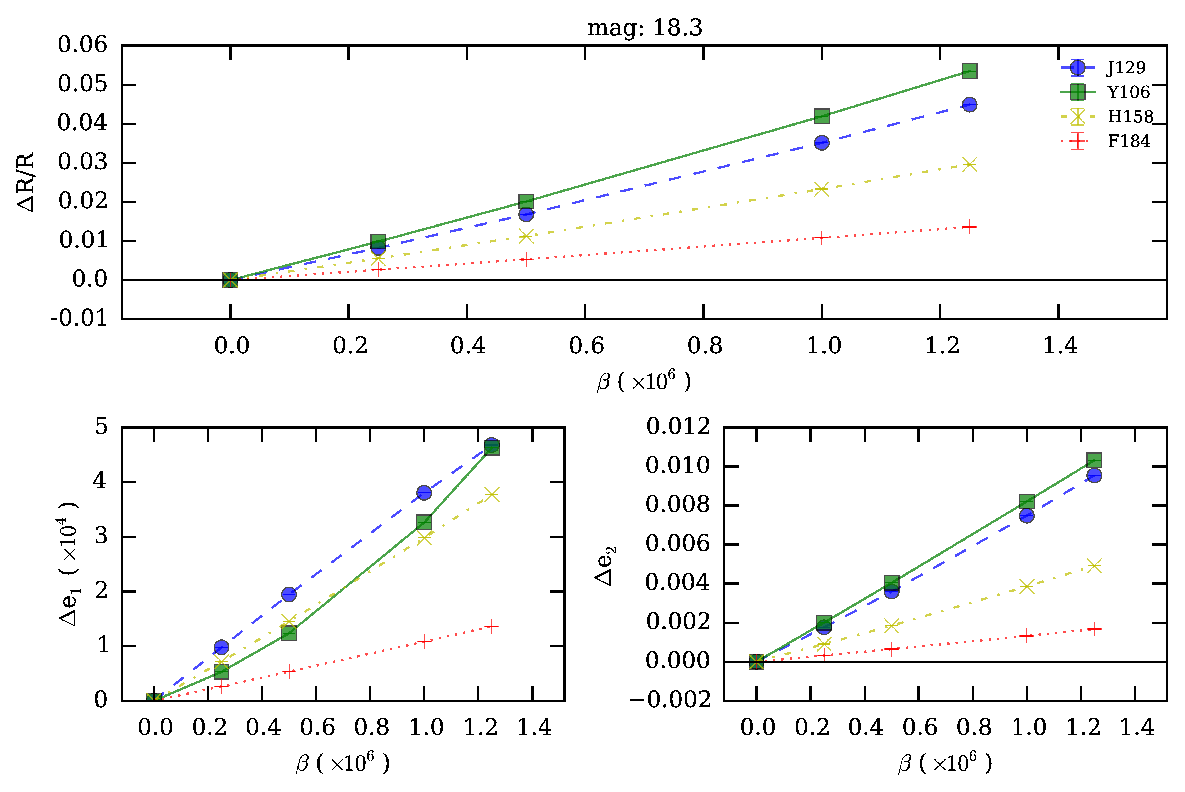
\includegraphics[page=1]{plots/f2.eps}}
\caption{Impact of spatial variability in the $\beta$ parameter,  measuring the standard deviation over $M=100$ realizations in $\Delta e_1$,  $\Delta e_1$, and $\Delta e_1$  as a function of the standard deviation $ \sigma_{\beta_0}$}
\label{f2}
\end{figure}

Fig. \ref{f3} shows the fractional change in PSF size and the absolute error in PSF ellipticity as a function of the mean nonlinearity parameter $\beta$, for different bandpass filters at fixed AB magnitude of 18.3 in each band, consistent with the magnitude of brightest stars that will be usable for the HLS. The effect depends on flux, and hence its amplitude is the largest in the Y106 bandpass filter (\emph{c.f.}, Table 1). We note that the flux in the other bands will depend on the stellar spectral energy distribution (SED), and we would need to specify a particular SED to go from the reference band to other bands. For simplicity, we are performing our calculations based on a grid of AB magnitudes in different bands, as calculated by \gs.

\begin{figure}[!h]
\centering
\resizebox{\hsize}{!}{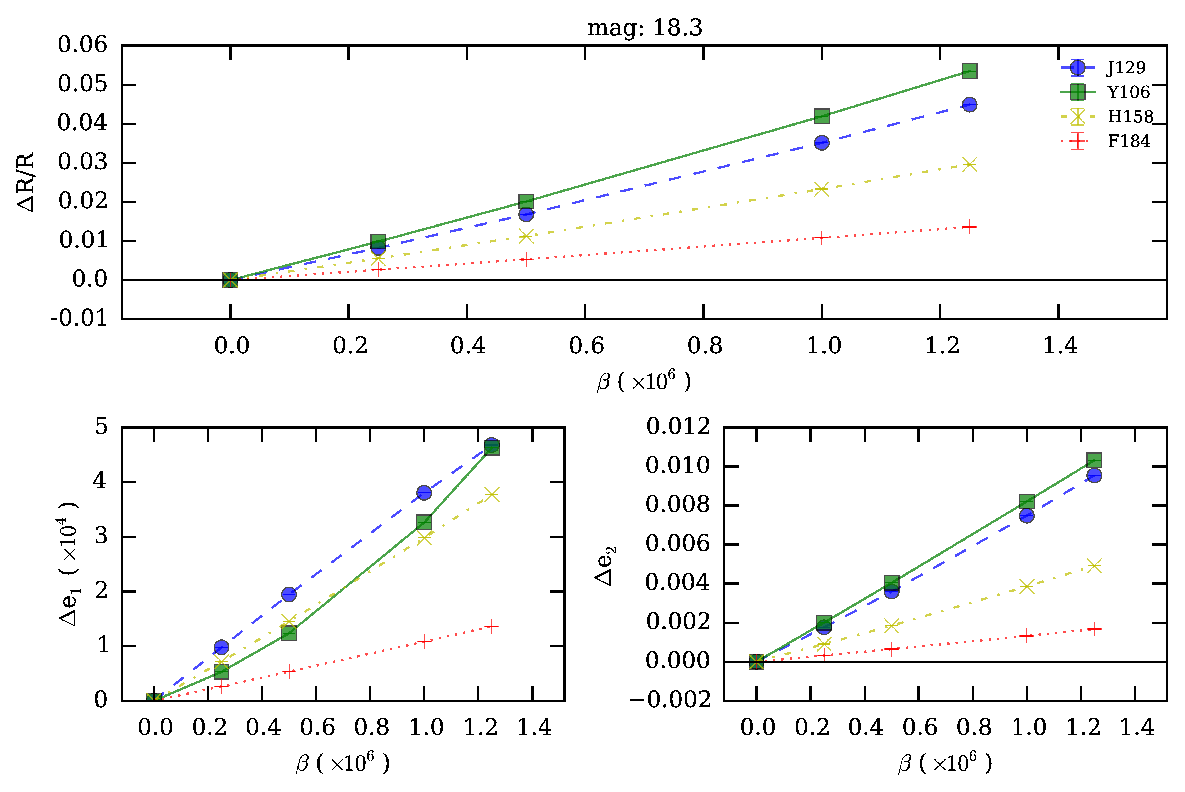
\includegraphics[page=1]{plots/f3.eps}}
\caption{Fractional error in PSF size (upper panel) and absolute error in PSF ellipticity components (lower panels) as a function of the mean nonlinearity parameter $\beta$ for the \wfa\ PSF, in four the four HSL filters (J129, Y106, H158, and F184), and an AB magnitude of 18.3 (similar plots were found for other magnitude values). In each plot, the nominal value for the nonlinearity model parameter $\beta_0$ is located at the second point from the origin. Each point is the mean over 100 realizations of uniformly distributed random centroid shifts within the high resolution images($N=3$), and the associated error bars (too small to be seen) represent the standard deviation of the realizations.}
\label{f3}
\end{figure}
In this band, the mean nominal value of $\beta_0=5\times10^{-7}/\mathrm{e^-}$ induces errors in the size and ellipticity of about $2\times10^{-2}$ and $4\times10^{-3}$ respectively, larger than the required values of $10^{-3}$ and $4.5\times10^{-4}$ on the knowledge of the size and ellipticity of the PSF in order not to bias cosmological parameter inferences from WL experiments (Section \S1). As the $\beta$ parameter is increased, the amplitude of the errors increases approximately in a linear manner within the domain of $\beta$ values considered. 
%It is possible to obtain a more general relationship between $\Delta R/R$ (or $\Delta e$), $\beta$, and object flux for each band by Taylor expanding to first order around any given value in $\beta$ and plotting the slope as a function of magnitude. 
\begin{figure}[!h]
\centering
\resizebox{\hsize}{!}{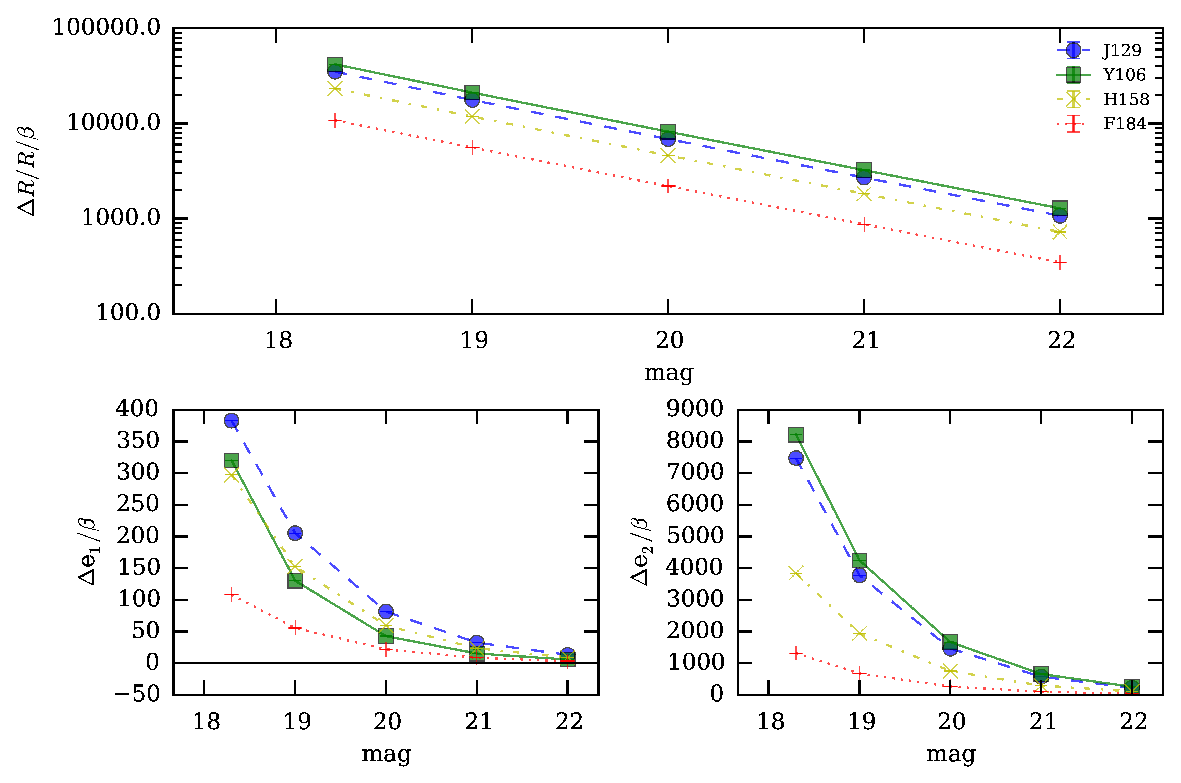
\includegraphics[page=1]{plots/f4.eps}}
\caption{Fractional error in PSF size and absolute error in PSF ellipticity components normalized by the NL parameter $\beta$, as a function of magnitude for the four HSL filters (J129, Y106, H158, and F184). The ordinate axis in each plot represents the slope of the linear relationships in Fig. \ref{beta}, derived by linear fitting of points around the vicinity of $\beta_0$ in each curve of that figure.}
\label{f4}
\end{figure}
Since $\Delta R/R$ and $\Delta e$ are approximately linear in $\beta$, we can condense this information by simply plotting the slope for various filters and star magnitudes. This is shown in Fig. \ref{f4}, which shows $\Delta R/R/\beta$ and $\Delta e/\beta$ (the slopes in Fig. \ref{beta}) vs $m$ for each of the four filters of the HLS. From Fig. \ref{f4}, it is possible to estimate the precision to which $\beta$ would have to be calibrated in order to limit the relative size and ellipticity bias of a star with a given magnitude. In particular, letting $(\beta - \beta_0)/\beta_0 \equiv \Delta \beta / \beta_0$ represent the fractional error in the measurement of a given value of $\beta_0$, we have: 
\begin{align}
\frac{\Delta R/R}{\Delta \beta} = c \ \ \ \  \Rightarrow \ \ \ \ \frac{\Delta R/R}{\Delta \beta / \beta_0} = c \beta_0  \ \ \   \Rightarrow \ \ \
\frac{\Delta \beta}{\beta_0} = \frac{\Delta R/R}{c \beta_0}
\label{calib}
\end{align}
In Eq.\ref{calib}, $c$ represents the ordinate value in Fig. \ref{f4} for a given magnitude, and we have replaced $\Delta R/R/\beta$ by $\Delta R/R/ \Delta \beta$ since the linearity in the bias in $\Delta R/R$ and $\Delta e$ vs $\beta$ for all magnitudes makes the choice of the expansion point of the approximation by Taylor expansion unimportant (\emph{i.e.}, it does not matter if the expansion is around $\beta=0$ or $\beta=\beta_0$). An analogous equation to Eq. \ref{calib} can be written for the error in the ellipticity if $\Delta R/R$ is replaced by $\Delta e$. 

Under these conditions, Fig. \ref{magnitude} shows that to limit the bias of $\Delta R/R$ ($\Delta e$) in the H158 band to $10^{-4}$  ($4.7\times 10^{-5}$)\textemdash about $10\%$ of the estimated \wf\ error budgets, $\beta$ must be calibrated to $\sim1\%$ ($\sim 2.4\%$) (using $c\sim4\times10^3 \mathrm{e^-}$ at $m=18.3$ from the upper panel of Fig. \ref{magnitude}, $c\sim1300$ at $m=18.3$ from the lower right panel of the same figure, and $\beta_0=5\times10^{-7}/\mathrm{e^-}$) for the brightest stars usable by the HLS. Notice that the numbers for the tolerable errors on the size and ellipticity of the PSF are estimates; however, Eq. \ref{calib} and Fig. 3 can now be used to derive WFIRST detector requirements once true PSF requirements are chosen.


\section{Conclusion}
\label{Conclusion}
We have used the \wfa\ module in \gs\ to study the impact on PSF measurement for weak lensing science due to the non-linearity in the conversion of charge to voltage in near-infrared hybrid CMOS detectors (such as those that will be used in the Wide Field Imager of the \wfa\ mission). The PSF profiles created by {\tt{galsim.wfirst}} posses several of the design characteristics of the expected PSF of the mission, such as optical aberrations and pixel scale. We have also used the \wfa\ Exposure Time Calculator in weak lensing mode to assign the PSF profiles fluxes per pixel consistent with the expected brightness of the HLS. 

Voltage non-linearity\textemdash as studied in this work\textemdash encompasses the linearity due to the shrinking of the depletion region at the p-n junction as charge accumulates, and the deviation from linearity originating in the multiplexer gain. It depends on the total integrated signal (fluence), and it is more dominant at high signals than other types of non-linearity such as reciprocity failure, which dominates at lower signals. As such, NL will tend to attenuate the bright stars that are usually used for PSF estimation, introducing errors when de-convolving the PSF at the interpolated galaxy positions.

To model NL, we have used a single, one-parameter transfer function quadratic in the mean signal $\langle Q \rangle$ (Eq. \ref{NL}). In principle, different pixels can have different underlying non-linearity coefficients which in practice can be difficult to measure with sufficient precision, so the mean response is usually measured. In our simulations, we have assumed that each individual pixel has a different non-linearity coefficient that follows a Normal distribution, and we have verified that the results obtained in this way do not differ from those obtained by using the same mean NL coefficient for all pixels. This implies that using the mean pixel behavior to calibrate NL will not introduce significant biases in the measurement of PSF properties for WL science.  However, while it is more practical to measure a single mean NL calibration curve instead of one for each pixel, one must be careful to mask and exclude from the average those pixels that might reach digital saturation before entering the NL regime. This situation arises due to the DC offsets which are intrinsic to the readout circuit and which vary from pixel to pixel. 

We have studied the consequences of NL in isolation by using the relationship in Eq.\ref{NL}, not considering other sensor effects, and neglecting sources of noise such as zodiacal background, thermal emission, and read noise (which would produce a negligible contribution). We have used the metrics $\Delta R/R$ and $\Delta e$ to assess the impact of NL on PSF size and ellipticity, which have to be controlled to $\sim O(10^{-4})$ or better, for different values of the parameter space at hand ($\beta$, PSF magnitude, and bandpass filters to be used in \wfa\ WL analyses). In particular, our simulations show that the effects of NL are the largest in the J129 band and linear with the nonlinearity parameter $\beta$. For the  nominal value $\beta_0$ assumed in this work\textemdash obtained from measurements of a H2RG detector\textemdash NL induces errors in PSF size and shape comparable to what is tolerable by accurate WL measurements. For a particular set of estimated requirements on PSF size and ellipticity ($10^{-4}$  and $4.7\times 10^{-5}$, respectively), we find that the mean $\beta$ should be calibrated to about $1\%$ to $2.4\%$. However, the results derived in this study (Eq. \ref{calib} and Fig. 3) can be used to derive requirements on NL for the \wfa\ detectors for a different set of tolerances on PSF properties. It is important to note that new measurements on the actual H4RG detector that will be used by the \wf\ imager will have to be performed in order to determine the mean value of $\beta$ and its dispersion.

Non-linearity measurements are usually performed by looking at signal as a function of exposure time at a constant flux (and subtracting dark frames at the appropriate times), which is sensible to any gain dependence on fluence. These measurements are normally subject to other effects such as inaccuracies in the readout time, persistence, reciprocity failure, and time-dependent changes in the electronic offset due to self-heating effects in the multiplexer. Despite these challenges, the mean non-linearity signal can usually be characterized to a precision of 5\textendash10$\%$. Thus it is not obvious that a typical NL calibration program will be sufficient for WL with \wf\ without more careful study and error budgeting.
Validation tests will therefore be crucial through the use of a facility such as the 
Precision Projector Laboratory (PPL, \citealt{seshadri13}, \citealt{shapiro13})\footnote{The PPL is a joint project between NASA Jet Propulsion Laboratory and Caltech which characterizes image sensors using laboratory emulations of astronomical data.} to ensure that voltage nonlinearity in the \wf\ H4RG detectors can be calibrated to the levels demanded by WL science.\\

% DC offsets which are intrinsic to the readout circuit and which vary from pixel to pixel

%Something to keep in mind is that different pixels could have different underlying linearity coefficients but in practice its very hard to measure this with sufficient precision so we find ourselves using the mean pixel behavior and accepting a degree of mismatch between a pixel and the mean.  Does this matter?   Maybe not, but I think this is a good example where simulation is better than measurement since you can test whether biases are introduced.   

%Nonlinear gain V(Q) depends on fluence (total charge/pixel), not flux (charge/pixel/second).  We can't use SPR to measure nonlinear gain because there's no independent measurement of Q.  We're not really measuring flux in the reciprocity failure case either, just a signal decay.

We thank Chris Hirata and the WFIRST detector requirements working group for useful discussions. AAP is supported by the Jet Propulsion Laboratory. CS and JR are being supported in part by the Jet Propulsion Laboratory. The research was carried out at the Jet Propulsion Laboratory, California Institute of Technology, under a contract with the National Aeronautics and Space Administration.

\copyright\ 2016. All rights reserved.

%\section*{Appendix}

%The parameters used in the weak lensing mode of the Exposure Time Calculator (ETC-WL) to obtain the flux (in electrons) at AB magnitude 20 for each of the four bands simulated (J129, W149, H158, and F184) are as follows (see \citealt{spergel15} and \citealt{hirata12}): 
%\begin{multicols}{2}
%\begin{enumerate}
%\item[\textemdash] telescope configuration: 0 (generic)
%\item[\textemdash] aperture outer diameter: 2.4 m
%\item[\textemdash] central obscuration: 0.3
%\item[\textemdash] pixel scale: 0.11 arcsec/pix
%\item[\textemdash] throughput: 0.8
%\item[\textemdash] RMS wavefront error: 0.05 $\mu$m
%\item[\textemdash] detector type: 2 (H4RG)
%\item[\textemdash] pointing jitter: 0.00 arcsec per axis
%\item[\textemdash] minimum wavelength: \emph{filter dependent} (see Table 1)
%\item[\textemdash] maximum wavelength: \emph{filter dependent} (see Table 1)
%\item[\textemdash] filter throughput: 0.99  
%\item[\textemdash] single exposure time: 174 s
%\item[\textemdash] readnoise floor: 0.0 e$^{-}$/pix/s
%\item[\textemdash] dark current: 0.0 e$^{-}$/pix/s
%\item[\textemdash] (heliocentric) ecliptic latitude: -30 deg
%\item[\textemdash] galactic redening E(B-V): 0.03 mag
%\item[\textemdash] number of exposures: 9 ($N=3$) 
%\item[\textemdash] minimum resolution factor R: 0.425
%\item[\textemdash] maximum ellipticity error: 0.2
%\end{enumerate}
%\end{multicols}


%?Nonlinearity? includes nonlinear conversion gain (e-/ADU) and the ?brighter-fatter effect?. Postdoc Andres Plazas-Malagon is calculating the effects of these on shape measurement with WFIRST.
%Weak lensing scientists typically assume that nonlinear conversion gain (NL) will be sufficiently calibrated.  This was based on
%Experience with CCDs, not CMOS
%Previous, less stringent shape measurement requirements
%Top plot shows the change in PSF size DR/R vs. star magnitude for a single NL parameter b (quadratic term) in various filters.  For a nominal b=3.6E-7, NL biases the size of the brightest useable stars in the High Latitude Survey by a few \%.
%Bottom plot shows general relationship between size bias and b. To limit relative size bias of the brightest stars to ~10-4, b must be calibrated to better than 1\%.




\acknowledgments
%We thank...
\bibliographystyle{plainnat}
\bibliography{bias_from_NL}

\end{document}